Establishment of the threshold at 40 is based on human challenge studies from the 1960s in which volunteers were either randomised to received vaccine or not, or were challenged with virus \citep{Hobson;1972}. Blood samples were collected pre-challenge. For vaccinated individuals, challenge occurred at least 14 days after vaccination. Nasal swabs taken 48-hours after challenge were used to determine infection by virus culture, and for unvaccinated volunteers challenged with live virus, infection was additionally indicated by pre-to-post-challenge sero-conversion (4-fold rise in titre). In both cases, the protective titre was estimated from the pre-challenge geometric mean titre for uninfected participants.

While challenge studies permit close observation of participant responses to infection under highly controlled conditions, the infectious dose administered may be unnaturally high. Several observational studies have been established to understand influenza transmission in more realistic conditions. In these studies, participants are determined to be at risk of infection because one or more of their close contacts (i.e. household members) has been identified as influenza-infected or because influenza has been known to be circulating.  Infection may be determined by laboratory testing of respiratory samples, or, if unvaccinated, by sero-conversion. In this paper, we will illustrate our findings using two established household studies.

The differences between challenge studies and observational studies are depicted in Figure \ref{fig:study-design}

\begin{figure}[htp]
    \centering
    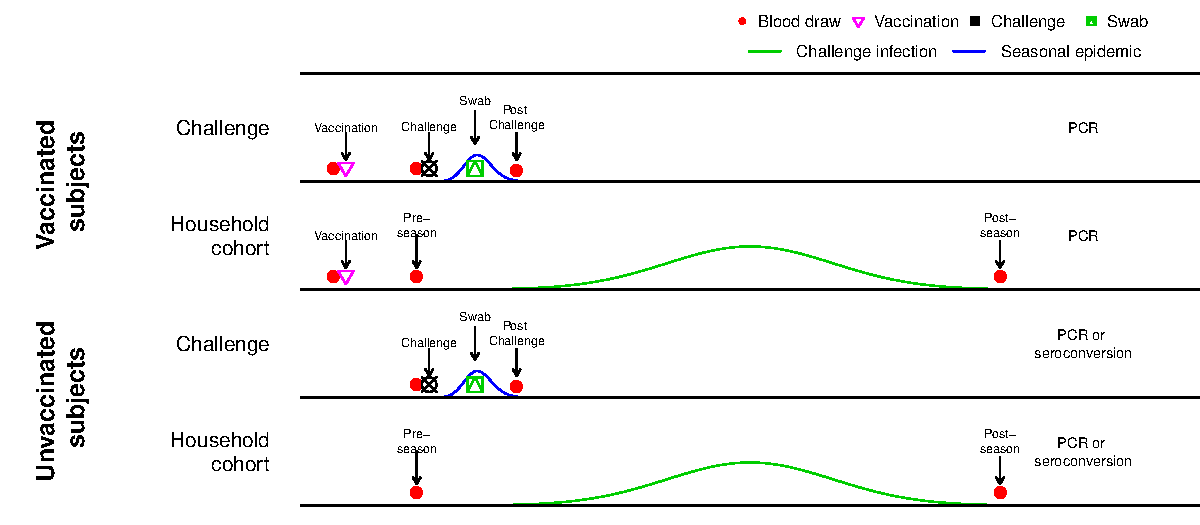
\includegraphics[width=\linewidth]{../fig-studies/fig-studies.pdf}
    \caption{\footnotesize
        Example study designs for the estimation of protective titres.
    }
    \label{fig:study-design}
\end{figure}
